%%%% main.tex, 2022/08/10, 2.5
%%%% Copyright (C) 2020 Vinicius Pegorini (vinicius@utfpr.edu.br)
%%
%% This work may be distributed and/or modified under the conditions of the
%% LaTeX Project Public License, either version 1.3 of this license or (at your
%% option) any later version.
%% The latest version of this license is in
%%   http://www.latex-project.org/lppl.txt
%% and version 1.3 or later is part of all distributions of LaTeX version
%% 2005/12/01 or later.
%%
%% This work has the LPPL maintenance status `maintained'.
%%
%% The Current Maintainer of this work is Vinicius Pegorini.
%%
%% This work consists of the files utfprpb.cls, utfprpb.tex, and
%% utfprpb-dados.tex.
%%
%% The Current Maintainer of this work is Vinicius Pegorini.
%% Updated by:
%% - Marco Aurélio Graciotto Silva;
%% - Rogério Aparecido Gonçalves;
%% - Luiz Arthur Feitosa dos Santos.
%%
%% This work consists of the files utfpr.cls, main.tex, and
%% variaveis.tex.
%% A brief description of this work is in readme.md.

%% ####################################################
%%
%% >> Atenção - Leia isso antes de usar esse template<< 
%%
%% Esse template foi desenvolvido por professores,  com a intenção de ajudar os alunos com as entregas na biblioteca. Não há uma equipe especializada e dedicada mantendo tal template, mas sim professores trabalhando além das suas funções básicas, que são: ensino, pesquisa e extensão.
%
%% Também os mantenedores deste template não são especializados em LaTeX, muito menos em normas da ABNT. Todos que contribuíram com o template fizeram isso visando deixá-lo o mais próximo possível das normas da ABNT e das regras, anseios e expectativas da biblioteca da UTFPR. É muito importante entender que os desenvolvedores do template não têm relação direta com a biblioteca ou com a ABNT. Ou seja, não são os desenvolvedores do template que ditam as regras e normas dos textos que devem ser entregues à biblioteca.

%%É válido informar também, que como não há uma equipe dedicada e especializada, o tempo para colaborar com o template é curto. Desta forma, pode ser que não sejam empregadas as melhores técnicas, métodos e ferramentas para o desenvolvimento do template. Também pode acontecer do template não atender completamente todos os anseios e exigências da ABNT e da biblioteca, pois por exemplo, muitas regras de redação possuem questões interpretativas. Assim, o template sempre estará em contínua evolução e seria extremamente interessante que as pessoas (alunos,  professores,  técnicos e entusiastas) colaborarem com a evolução do template. Toda ajuda será bem vinda! Isso pode ser feito enviando e-mail para os desenvolvedores, desta forma, assim que possível esses vão tentar melhorar o template.

%%O template é apenas mais uma ferramenta para o desenvolvimento de trabalhos para a biblioteca. Todavia, podem existir outros templates LaTeX. Assim como há templates em outros formatos, que não o LaTeX. O mais importante é que qualquer pessoa, utilizando a princípio qualquer ferramenta, pode desenvolver textos que atendem os requisitos da biblioteca apenas estudando, interpretando e seguindo as regras da UTFPR e da ABNT, que estão disponíveis na página Web da instituição. O template é só um facilitador.

%%Por fim,  é necessário entender que infelizmente o ambiente LaTeX pode ser complexo e gerar resultados distintos dependendo do: sistema operacional,  pacotes LaTeX utilizados,  configurações alteradas, editor utilizado, a forma que está sendo redigida textos, figuras,  etc. Assim não há como garantir que o resultado final será o esperado.  Dito tudo isso,  >>UTILIZE ESSE TEMPLATE POR SUA CONTA E RISCO<<. Os desenvolvedores e colaboradores deste template não se responsabilizam pelo resultado do uso deste template e se eximem de qualquer responsabilidade.

%###################################################


% Luiz - pdfa: inclusão do pdfa
\PassOptionsToPackage{
	pdfa
}{hyperref}

%% Classe e opções de documento
\documentclass[%% Opções
%% -- Opções da classe memoir --
  12pt,%% Tamanho da fonte: 10pt, 11pt, 12pt, etc.
  a4paper,%% Tamanho do papel: a4paper (A4), letterpaper (carta), etc.
  % fleqn,%% Alinhamento das equações à esquerda (comente para alinhamento centralizado)
  % leqno,%% Numeração das equações no lado esquerdo (comente para lado direito)
  oneside,%% Impressão dos elementos textuais e pós-textuais: oneside (anverso) ou twoside (anverso e verso, se mais de 100 p.)
  openright,%% Impressão da primeira página dos capítulos: openright (anverso), openleft (verso) ou openany (anverso e verso)
%% -- Opções da classe abntex2 --
  sumario = abnt-6027-2012,%% Formatação do sumário: tradicional (estilo tradicional) ou abnt-6027-2012 (norma ABNT 6027-2012)
  chapter = TITLE,%% Títulos de capítulos em maiúsculas (comente para desabilitar)
  % luiz - comentar section para ser minusculo
  %section = TITLE,%% Títulos de seções secundárias em maiúsculas (comente para desabilitar)
  % subsection = TITLE,%% Títulos de seções terciárias em maiúsculas (comente para desabilitar)
  % subsubsection = TITLE,%% Títulos de seções quartenárias em maiúsculas (comente para desabilitar),
%% -- Opções da classe utfprpgtex --
  pretextualoneside,%% Impressão dos elementos pré  -textuais: pretextualoneside (anverso) ou pretextualtwoside (anverso e verso)
  fontetimes,%% Fonte do texto: fontetimes (times), fontearial (arial) ou fontecourier (courier)
  % vinculoscoloridos,%% Cores nos vínculos (citações, arquivos, links, url, etc.) (comente para desabilitar)
  semrecuonosumario,%% Remoção do recuo dos itens no sumário (comente para adição do recuo, se estilo tradicional)
  usemakeindex,%% Compilação de glossários e índices utilizando makeindex (comente para desabilitar)
  % legendascentralizadas,%% Alinhamento das legendas centralizado (comente para alinhamento à esquerda)
  %aprovacaoestiloppg,%% Folha de aprovação do programa de pós-graduação no estilo do PPG (comente para estilo padrão)
  pardeassinaturas,%% Assinaturas na folha de aprovação em até duas colunas (comente para em uma única coluna)
  % linhasdeassinaturas,%% Linhas de assinaturas na folha de aprovação (comente para remover as linhas)
%% -- Opções do pacote babel --
  english,%% Idioma adicional para hifenização
  french,%% Idioma adicional para hifenização
  spanish,%% Idioma adicional para hifenização
  brazil,%% Idioma principal do documento (último da lista)
]{utfpr}%% Classe utfpr

% Luiz: pdfa: necessário para criar pdfa
\usepackage[a-3b,mathxmp]{pdfx}[2018/12/22] % você pode escolher entre a-1b, a-2b, a-3b - o template ainda não suporta o a-Xa de 

%%%% configuracoes.tex, 2022/05/02, 2.4a

%% ####################################################
%%
%% >> Atenção - Leia isso antes de usar esse template<< 
%%
%% Esse template foi desenvolvido por professores,  com a intenção de ajudar os alunos com as entregas na biblioteca. Não há uma equipe especializada e dedicada mantendo tal template, mas sim professores trabalhando além das suas funções básicas, que são: ensino, pesquisa e extensão.
%
%% Também os mantenedores deste template não são especializados em LaTeX, muito menos em normas da ABNT. Todos que contribuíram com o template fizeram isso visando deixá-lo o mais próximo possível das normas da ABNT e das regras, anseios e expectativas da biblioteca da UTFPR. É muito importante entender que os desenvolvedores do template não têm relação direta com a biblioteca ou com a ABNT. Ou seja, não são os desenvolvedores do template que ditam as regras e normas dos textos que devem ser entregues à biblioteca.

%%É válido informar também, que como não há uma equipe dedicada e especializada, o tempo para colaborar com o template é curto. Desta forma, pode ser que não sejam empregadas as melhores técnicas, métodos e ferramentas para o desenvolvimento do template. Também pode acontecer do template não atender completamente todos os anseios e exigências da ABNT e da biblioteca, pois por exemplo, muitas regras de redação possuem questões interpretativas. Assim, o template sempre estará em contínua evolução e seria extremamente interessante que as pessoas (alunos,  professores,  técnicos e entusiastas) colaborarem com a evolução do template. Toda ajuda será bem vinda! Isso pode ser feito enviando e-mail para os desenvolvedores, desta forma, assim que possível esses vão tentar melhorar o template.

%%O template é apenas mais uma ferramenta para o desenvolvimento de trabalhos para a biblioteca. Todavia, podem existir outros templates LaTeX. Assim como há templates em outros formatos, que não o LaTeX. O mais importante é que qualquer pessoa, utilizando a princípio qualquer ferramenta, pode desenvolver textos que atendem os requisitos da biblioteca apenas estudando, interpretando e seguindo as regras da UTFPR e da ABNT, que estão disponíveis na página Web da instituição. O template é só um facilitador.

%%Por fim,  é necessário entender que infelizmente o ambiente LaTeX pode ser complexo e gerar resultados distintos dependendo do: sistema operacional,  pacotes LaTeX utilizados,  configurações alteradas, editor utilizado, a forma que está sendo redigida textos, figuras,  etc. Assim não há como garantir que o resultado final será o esperado.  Dito tudo isso,  >>UTILIZE ESSE TEMPLATE POR SUA CONTA E RISCO<<. Os desenvolvedores e colaboradores deste template não se responsabilizam pelo resultado do uso deste template e se eximem de qualquer responsabilidade.

%###################################################

%% Pacotes carregados nas classes:
%%   memoir: abstract, appendix, array, booktabs, ccaption, chngcntr, chngpage, dcolumn, delarray, enumerate, epigraph, framed,
%%           ifmtarg, ifpdf, index, makeidx, moreverb, needspace, newfile, nextpage, parskip, patchcmd, setspace, shortvrb, showidx,
%%           tabularx, titleref, titling, tocbibind, tocloft, verbatim, verse.
%%   memoir (similares): crop, fancyhdr, geometry, sidecap, subfigure, titlesec.
%%   abntex2: babel, bookmark, calc, enumitem, ifthen, hyperref, textcase.
%%   utfprpgtex: abntex2cite, ae, algorithmic, amsmath, backref, breakurl, caption, cmap, color, eepic, epic, epsfig, etoolbox,
%%               fancyhdr, fix-cm, fontenc, glossaries, graphics, graphicx, helvet, hyphenat, indentfirst, inputenc, lastpage,
%%               morewrites, nomencl, sfmath, sistyle, substr, times, xtab.


%% Pacotes adicionais (\usepackage[options]{package})
\usepackage{bigdelim, booktabs, colortbl, longtable, multirow}%% Ferramentas para tabelas
\usepackage{amssymb, amstext, amsthm, icomma}%% Ferramentas para linguagem matemática
\usepackage{pifont, textcomp, wasysym}%% Símbolos de texto
\usepackage{lipsum}				% para geração de dummy text
\usepackage{subfig}             % para adicionar figuras lado a lado no texto                    
\usepackage{pdfpages}           % para adicionar documentos pdf ao trabalho
\usepackage{xspace}


% luiz: primeira letra maiúscula
% solução 1
%\usepackage{stringstrings}
%\newcommand{\firstcap}[1]{\caselower[e]{#1}\capitalize{\thestring}}

% solução 2 - não usei essa
% \usepackage[utf8]{inputenc}
% \usepackage{datatool-base}
% \usepackage{mfirstuc}

% Formatação do título da seção - primeira letra caixa alta e o resto em caixa baixa.
% \usepackage[explicit]{titlesec}
% \usepackage{lipsum}
% \titleformat{\section}{\normalfont}{\thesection}{1em}{\textbf{\firstcap{#1}}} % funciona mas apenas para o título da seção e não para o sumário (a configuração do sumário está mais para baixo

% luiz: define o underline colorido.
% https://github.com/abntex/abntex2-contrib/blob/master/customizacoes/pucminas/abntex2-pucminas.sty
% acabei não usando o black e o coloruline da solução do link

\usepackage[normalem]{ulem} % para o underline colorido na seção quaternária
\renewcommand*{\cftsubsubsectionfont}{\normalfont\uline} % underline no sumário
\setsubsubsecheadstyle{\ABNTEXsubsubsectionfont\ABNTEXsubsubsectionfontsize\ABNTEXsubsubsectionupperifneeded\uline} %underline no título da subsubsection

% luiz: bibliografia - opções

%% Comandos personalizados (\newcommand{name}[num]{definition})
\newcommand{\cpp}{\texttt{C$++$}}%% C++
\newcommand{\latex}{\LaTeX\xspace}%% LaTeX
\newcommand{\ds}{\displaystyle}%% Tamanho normal das equações
\newcommand{\bsym}[1]{\boldsymbol{#1}}%% Texto no modo matemático em negrito
\newcommand{\mr}[1]{\mathrm{#1}}%% Texto no modo matemático normal (não itálico)
\newcommand{\der}{\mr{d}}%% Operador diferencial
\newcommand{\deri}[2]{\frac{\der #1}{\der #2}}%% Derivada ordinária
\newcommand{\derip}[2]{\frac{\partial #1}{\partial #2}}%% Derivada parcial
\newcommand{\pare}[1]{\left( #1 \right)}%% Parênteses
\newcommand{\colc}[1]{\left[ #1 \right]}%% Colchetes
\newcommand{\chav}[1]{\left\lbrace #1 \right\rbrace}%% Chaves
\newcommand{\sen}{\operatorname{sen}}%% Operador seno
\newcommand{\senh}{\operatorname{senh}}%% Operador seno hiperbólico
\newcommand{\tg}{\operatorname{tg}}%% Operador tangente
\newcommand{\tgh}{\operatorname{tgh}}%% Operador tangente hiperbólico
\newcommand{\seqref}[1]{Equação~\eqref{#1}}%% Referência de uma única equação
\newcommand{\meqref}[1]{Equações~\eqref{#1}}%% Referência de múltiplas equações
\newcommand{\citep}[1]{\cite{#1}}%% Atalho para citação implícita
\newcommand{\citet}[1]{\citeonline{#1}}%% Atalho para citação explícita
\newcommand{\citepa}[1]{(\citeauthor{#1})}%% Atalho para citação implícita (somente autor)
\newcommand{\citeta}[1]{\citeauthoronline{#1}}%% Atalho para citação explícita (somente autor)
\newcommand{\citepy}[1]{(\citeyear{#1})}%% Atalho para citação implícita (somente ano)
\newcommand{\citety}[1]{\citeyear{#1}}%% Atalho para citação explícita (somente ano)

\newcommand{\fonteTexto}[1]{\renewcommand{\familydefault}{#1}}

% Define o caminho das figuras
\graphicspath{{figuras/}}

% Define a fonte ara helvet que é uma fonte similar à Arial, se for usar a Arial tem que mudar o compilador para XeLaTex, mas ai tem que arrumar os erros: https://latex.org/forum/viewtopic.php?t=25998
%\usepackage{helvet}
%\renewcommand{\familydefault}{\sfdefault}
%\usepackage{times} % para fonte time new roman
%\usepackage{pslatex} % ou essa aqui...

%\usepackage{titlesec}

%% Configuração de glossário
% \usepackage[portuguese]{nomencl}
% \usepackage[nogroupskip,nonumberlist,nopostdot,nohypertypes={acronym}]{glossaries}
% \makenoidxglossaries
\usepackage{glossaries}
\makeglossaries

% para siglas em português
\newcommand{\siglaPt}[2]
{
 \newglossaryentry{#1}{
  name=#1,
  description={#2},
  first={#2 (#1)},
  long={#2}
 }  
}

% para siglas de língua estrangeira, nessas a descrição longa fica em itálico.
\newcommand{\siglaIt}[2]
{
 \newglossaryentry{#1}{
  name=#1,
  description={\textit{#2}},
  first={\textit{#2} ({#1})},
  long={\textit{#2}}
 }  
}

%% luiz - para fazer os avisos
\usepackage{tcolorbox}

% use para criar caixas de avisos, pode ser utilizado para fazer anotações de tarefas indicadas pelo orientador/banca.
% \caixa{Atenção}{texto...}
\newcommand{\caixa}[2]{
\begin{tcolorbox}[colback=red!5!white,colframe=red!45!white, title = #1, fonttitle=\bfseries]
#2
\end{tcolorbox}
}

% Luiz - Linhas órfãs e viúvas
\widowpenalty=10000
\clubpenalty=10000

% Luiz - Caption do tamanho da Tabela
%\usepackage[width=1\textwidth]{caption}

% Luiz - configurar a margem dos itens
\setlength{\leftmargini}{1.5cm}
\setlength{\leftmarginii}{1.5cm}


%% Arquivo de dados do modelo de documento LaTeX para produção de trabalhos acadêmicos da UTFPR
%%%% variaveis.tex, 2022/05/02, 2.4a
%%%% Copyright (C) 2020 Vinicius Pegorini (vinicius@utfpr.edu.br)
%%
%% This work may be distributed and/or modified under the conditions of the
%% LaTeX Project Public License, either version 1.3 of this license or (at your
%% option) any later version.
%% The latest version of this license is in
%%   http://www.latex-project.org/lppl.txt
%% and version 1.3 or later is part of all distributions of LaTeX version
%% 2005/12/01 or later.
%%
%% This work has the LPPL maintenance status `maintained'.
%%
%% The Current Maintainer of this work is Vinicius Pegorini.
%% Updated by:
%% - Marco Aurélio Graciotto Silva;
%% - Rogério Aparecido Gonçalves;
%% - Luiz Arthur Feitosa dos Santos.
%%
%% This work consists of the files utfpr.cls, main.tex, and
%% variaveis.tex.
%%
%% A brief description of this work is in readme.txt.

%% ####################################################
%%
%% >> Atenção - Leia isso antes de usar esse template<< 
%%
%% Esse template foi desenvolvido por professores,  com a intenção de ajudar os alunos com as entregas na biblioteca. Não há uma equipe especializada e dedicada mantendo tal template, mas sim professores trabalhando além das suas funções básicas, que são: ensino, pesquisa e extensão.
%
%% Também os mantenedores deste template não são especializados em LaTeX, muito menos em normas da ABNT. Todos que contribuíram com o template fizeram isso visando deixá-lo o mais próximo possível das normas da ABNT e das regras, anseios e expectativas da biblioteca da UTFPR. É muito importante entender que os desenvolvedores do template não têm relação direta com a biblioteca ou com a ABNT. Ou seja, não são os desenvolvedores do template que ditam as regras e normas dos textos que devem ser entregues à biblioteca.

%%É válido informar também, que como não há uma equipe dedicada e especializada, o tempo para colaborar com o template é curto. Desta forma, pode ser que não sejam empregadas as melhores técnicas, métodos e ferramentas para o desenvolvimento do template. Também pode acontecer do template não atender completamente todos os anseios e exigências da ABNT e da biblioteca, pois por exemplo, muitas regras de redação possuem questões interpretativas. Assim, o template sempre estará em contínua evolução e seria extremamente interessante que as pessoas (alunos,  professores,  técnicos e entusiastas) colaborarem com a evolução do template. Toda ajuda será bem vinda! Isso pode ser feito enviando e-mail para os desenvolvedores, desta forma, assim que possível esses vão tentar melhorar o template.

%%O template é apenas mais uma ferramenta para o desenvolvimento de trabalhos para a biblioteca. Todavia, podem existir outros templates LaTeX. Assim como há templates em outros formatos, que não o LaTeX. O mais importante é que qualquer pessoa, utilizando a princípio qualquer ferramenta, pode desenvolver textos que atendem os requisitos da biblioteca apenas estudando, interpretando e seguindo as regras da UTFPR e da ABNT, que estão disponíveis na página Web da instituição. O template é só um facilitador.

%%Por fim,  é necessário entender que infelizmente o ambiente LaTeX pode ser complexo e gerar resultados distintos dependendo do: sistema operacional,  pacotes LaTeX utilizados,  configurações alteradas, editor utilizado, a forma que está sendo redigida textos, figuras,  etc. Assim não há como garantir que o resultado final será o esperado.  Dito tudo isso,  >>UTILIZE ESSE TEMPLATE POR SUA CONTA E RISCO<<. Os desenvolvedores e colaboradores deste template não se responsabilizam pelo resultado do uso deste template e se eximem de qualquer responsabilidade.

%###################################################

%% Documento
%% Luiz: Define a fonte do texto da monografia
\fonteTexto{\sfdefault} % utilize \rmdefault para Times New Roman ou \sfdefault para Arial
\TipoDeDocumento{Trabalho de Conclusão de Curso de Graduação}%% Tipo de documento: "Tese", "Dissertação" ou "Trabalho de Conclusão de Curso de Graduação", "Estágio Supervisionado"
\NivelDeFormacao{Bacharelado}%% Nível de formação: "Doutorado", "Mestrado", "Bacharelado" ou "Tecnólogo" - ATENÇÃO, isso será utilizado para alterar a formatação do trabalho, pois pode haver formatações distintas dependendo o nível/tipo de trabalho.


%% luiz
% Template LaTex criado pelo Departamento Acadêmico de Computação (DACOM)
% da Universidade Tecnológica Federal do Paraná - Campus Campo Mourão (UTFPR-CM)
% Criado e alterado pelos professores:
% - Marco Aurélio Graciotto Silva
% - Rogério Aparecido Gonçalvez
% - Luiz Arthur Feitosa dos Santos
% Esse template utiliza a licença CC BY:
% Esta licença permite que outros distribuam, remixem, adaptem e criem a partir deste trabalho, mesmo para fins comerciais, desde que atribuam o devido crédito pela criação original.
% https://creativecommons.org/licenses/by/4.0/deed.pt_BR

% Dados do curso. Caso seja BCC:
\program{Curso de Bacharelado em Ciência da Computação}
\programen{Undergradute Program in Computer Science}
\degree{Bacharel}
\degreearea{Ciência da Computação}
% Caso seja TSI:
% \program{Curso Superior de Tecnologia em Sistemas para Internet}
% \programen{Undergradute Program in Tecnology for Internet Systems}
% \degree{Tecnólogo}
% \degreearea{Tecnologia em Sistemas para Internet}


% Dados da disciplina. Escolha uma das opções e a descomente:
% TCC1:
%\goal{Proposta de Trabalho de Conclusão de Curso de Graduação}
%\course{Trabalho de Conclusão de Curso 1}
% TCC2:
 \goal{Trabalho de Conclusão de Curso de Graduação}
 \course{Trabalho de Conclusão de Curso 2}


% Dados do TCC (precisa alterar)
\author{Breno Farias da Silva}  % Seu nome
\authorbib{Silva, João da} % Seu nome para referência bibliográfica (Sobrenome, Nome)
\title{Teorema CAP em Sistemas Distribuídos: Uma Revisão Sistemática dos Princípios} % Título do trabalho
\titleen{CAP Theorem in Distributed Systems: A Systematic Review of the Principles} % Título traduzido para inglês
\advisor{Nome Orientador completo e título} % Nome do orientador. Lembre-se de prefixar com "Prof. Dr.", "Profª. Drª.", "Prof. Me." ou "Profª. Me."}
% Se não houver corientador, comente a linha a baixo
\coadvisor{Nome Orientador completo e título} % Nome do coorientador, caso exista. Caso não exista, comente a linha.
\depositshortdate{2023} % Ano em que depositou este documento
\approvaldate{19/maio/2023}

% Dados do curso que não precisam de alteração
\university{Universidade Tecnológica Federal do Paraná}
\universityen{Federal University of Technology -- Paraná}
\universitycampus{Campus Campo Mourão}
\universityunit{Departamento Acadêmico de Computação}
\address{Campo Mourão}
\addressen{Campo Mourão, PR, Brazil}
\documenttype{Monografia}
\documenttypeen{Monograph}
\degreetype{Graduação}

\evalboardmember{Nome completo e por extenso do Membro 1}{Título (especialização, mestrado, doutorado}{Nome completo e por extenso da instituição a qual possui vínculo}
\evalboardmember{Nome completo e por extenso do Membro 2}{Título (especialização, mestrado, doutorado}{Nome completo e por extenso da instituição a qual possui vínculo}
\evalboardmember{Nome completo e por extenso do Membro 3}{Título (especialização, mestrado, doutorado}{Nome completo e por extenso da instituição a qual possui vínculo}
\evalboardmember{Nome completo e por extenso do Membro 4}{Título (especialização, mestrado, doutorado}{Nome completo e por extenso da instituição a qual possui vínculo}

%% Palavras-chave e keywords
%% ATENÇÃO - você deve indicar a quantidade de palavras chaves para o template LaTeX utilizar o pontuação correta!
\NumeroDePalavrasChave{5}%% Número de palavras-chave (máximo 5)
%% Atenção - por enquanto o template não está suportando acentos normais na palavra chave, por isso caso a palavra tenha acento, você deve utilizar o estilo antigo do LaTeX, sendo os acentos: á - \'a  é - \'e   â - \^a  ê - \^e  à - \`a  ä - \"a  ç - \c{c}
\PalavraChaveA{Teorema CAP}%% Palavra-chave A
\PalavraChaveB{Sistemas Distribu\´idos}%% Palavra-chave B
\PalavraChaveC{Consist\^encia}%% Palavra-chave C
\PalavraChaveD{Disponibilidade}%% Palavra-chave D
\PalavraChaveE{Toler\^ancia a Parti\c{c}\~oes}%% Palavra-chave E
%% Exemplo de como utilizar acentos na Palavra-chave:
% \PalavraChaveA{ol\'a}%% Olá
%\PalavraChaveB{voc\^e}%% você
%\PalavraChaveC{\`a}%% à
%\PalavraChaveD{a\c{c}\~ao}%% ação
%\PalavraChaveE{arg\"uir}%% argüir


%% ATENÇÃO - você deve indicar a quantidade de keywords para o template LaTeX utilizar o pontuação correta!
\NumeroDeKeywords{5}%% Número de keywords (máximo 5)
\KeywordA{Keyword 1}%% Keyword A
\KeywordB{Keyword 2}%% Keyword B
\KeywordC{Keyword 3}%% Keyword C
\KeywordD{Keyword 4}%% Keyword D
\KeywordE{Keyword 5}%% Keyword E


% É obrigatório o uso de uma licença Creative Commons (CC) nos trabalhos de TCC pelos cursos ligados a DACOM da UTFPR-CM.
% Veja: http://portal.utfpr.edu.br/biblioteca/trabalhos-academicos/docentes/procedimento-de-entrega-graduacao

% Sendo assim, escolha com o seu orientador uma das licenças CC a seguir: 

% CC BY: Esta licença permite que outros distribuam, remixem, adaptem e criem a partir deste trabalho, mesmo para fins comerciais, desde que atribuam o devido crédito pela criação original. Essa é a menos restritiva.
\licenca{ccby}

% CC BY CA: Esta licença permite que outros remixem, adaptem e criem a partir deste trabalho, mesmo para fins comerciais, desde que atribuam o devido crédito e que licenciem as novas criações sob termos idênticos.
%\licenca{ccbysa}

% CC BY ND: Esta licença permite a redistribuição, comercial e não comercial, desde que o trabalho seja distribuído inalterado e no seu todo, com crédito ao autor.
%\licenca{ccbynd}

% CC BY NC: Esta licença permite que outros remixem, adaptem e criem a partir deste trabalho para fins não comerciais, e embora os novos trabalhos tenham de atribuir o devido crédito e não possam ser usados para fins comerciais, os trabalhos derivados não têm que serem licenciados sob os mesmos termos.
%\licenca{ccbync}

% CC BY NC SA: Esta licença permite que outros remixem, adaptem e criem a partir deste trabalho para fins não comerciais, desde que atribuam ao autor o devido crédito e que licenciem as novas criações sob termos idênticos.
%\licenca{ccbyncsa}

% CC BY NC ND: Esta licença só permite que outros façam download do trabalho e o compartilhe desde que atribuam crédito ao autor, mas sem que possam alterá-los de nenhuma forma ou utilizá-los para fins comerciais. Essa é a mais restritiva.
%\licenca{ccbyncnd}

% Deixar sem licença - isso é aplicado apenas aos trabalhos que não são obrigados a ter licença. Na duvida verifique isso com o seu orientador e professor responsável pelo TCC. Para deixar o texto sem licença deixe o comando licença em brando ou deixe comentado.
%\licenca{}
% by DACOM/UTFPR-CM%% Realize as modificações pertinentes no arquivo "utfprpb-dados.tex"

%% Ferramenta para criação de índices
\makeindex%% Não comente esta linha

%% Ferramenta para criação de glossários
\makeglossaries%% Não comente esta linha
%%%% LISTA DE ABREVIATURAS E SIGLAS 
%%
%% Relação, em ordem alfabética, das abreviaturas (representação de uma palavra por meio de alguma(s) de sua(s) sílaba(s) ou
%% letra(s)), siglas (conjunto de letras iniciais dos vocábulos e/ou números que representa um determinado nome) e acrônimos
%% (conjunto de letras iniciais dos vocábulos e/ou números que representa um determinado nome, formando uma palavra pronunciável).
%%
%% Este arquivo para definição de abreviaturas, siglas e acrônimos é utilizado com a opção "glossaries" (pacote)

%% Abreviaturas: \abreviatura{rótulo}{representação}{definição}

\abreviatura{art.}{art.}{Artigo}
\abreviatura{cap.}{cap.}{Capítulo}
\abreviatura{sec.}{sec.}{Seção}

%% Siglas: \sigla{rótulo}{representação}{definição}

\sigla{abnt}{ABNT}{Associação Brasileira de Normas Técnicas}
\sigla{cnpq}{CNPq}{Conselho Nacional de Desenvolvimento Científico e Tecnológico}
\sigla{eps}{EPS}{\textit{Encapsulated PostScript}}
\sigla{pdf}{PDF}{Formato de Documento Portátil, do inglês \textit{Portable Document Format}}
\sigla{ps}{PS}{\textit{PostScript}}
\sigla{utfpr}{UTFPR}{Universidade Tecnológica Federal do Paraná}


%% LEIA:

%% Para usar o \gls, você deve colocar a sigla aqui em \sigla

%% ADICIONAR SIGLAS: Quando você inclui alguma sigla, pode ser necessário compilar umas duas vezes para essa aparecer na lista de siglas.

%% ATENÇÃO REMOVER SIGLAS: se você remover a sigla do seu texto (não for usar mais), você deve comentar essa aqui e remover os \gls{} dessa sigla (se não vai ficar aparecendo a sigla na lista). Em caso de ERRO, quando o LaTeX informa que você ainda tem a sigla no texto, mesmo que não tenha. Você deve limpar o cache - no OverLeaf, clique no erro, vá:
%  ->view error
%%   ->(role para baixo, até o final)
%%     ->e clique em Clear cached files


%% Acrônimos: \acronimo{rótulo}{representação}{definição}
%\acronimo{gimp}{Gimp}{Programa de Manipulação de Imagem GNU, do inglês \textit{GNU Image Manipulation Program}}
%% Entradas da lista de abreviaturas e siglas - Comente para remover este item
%%%% GLOSSÁRIO
%%
%% Relação de palavras ou expressões técnicas de uso restrito ou de sentido obscuro, utilizadas no texto, acompanhadas das
%% respectivas definições.

%% Entradas do glossário: \newglossaryentry{rótulo}{informações da entrada}

\newglossaryentry{pai}{%% Informações da entrada
  name        = {pai},
  plural      = {pais},
  description = {um exemplo de entrada pai que possui subentradas (entradas filhas)}
}

\newglossaryentry{componente}{%% Informações da entrada
  name        = {componente},
  plural      = {componentes},
  parent      = {pai},
  description = {um exemplo de uma entrada componente, subentrada da entrada chamada \gls{pai}}
}

\newglossaryentry{filho}{%% Informações da entrada
  name        = {filho},
  plural      = {filhos},
  parent      = {pai},
  description = {um exemplo de uma entrada filha (subentrada) da entrada chamada \gls{pai}. Trata-se de uma entrada irmã da entrada chamada \gls{componente}}
}

\newglossaryentry{equilibrio}{%% Informações da entrada
  name        = {equilíbrio da configuração},
  see         = [veja também]{componente},
  description = {uma consistência entre os \glspl{componente}}
}

\newglossaryentry{tex}{%% Informações da entrada
  name        = {\TeX},
  sort        = {TeX},
  description = {é um sistema de tipografia criado por Donald E. Knuth}
}

\newglossaryentry{latex}{%% Informações da entrada
  name        = {\latex},
  sort        = {LaTeX},
  description = {um conjunto de macros para o processador de textos \gls{tex}, utilizado amplamente para a produção de textos matemáticos e científicos devido à sua alta qualidade tipográfica}
}

\newglossaryentry{bibtex}{%% Informações da entrada
  name        = {Bib\TeX},
  sort        = {BibTeX},
  parent      = {latex},
  description = {um software de gerenciamento de referências para a formatação de listas de referências. A ferramenta Bib\TeX\ é normalmente usada em conjunto com o sistema de preparação de documentos do \gls{latex}}
}

\newglossaryentry{abntex2}{%% Informações da entrada
  name        = {\abnTeX},
  sort        = {abnTeX2},
  see         = {latex},
  description = {uma suíte para \gls{latex} que atende os requisitos das normas da Associação Brasileira de Normas Técnicas (ABNT) para elaboração de documentos técnicos e científicos brasileiros, como artigos científicos, relatórios técnicos, trabalhos acadêmicos como teses, dissertações, projetos de pesquisa e outros documentos do gênero}
}

\newglossaryentry{utfprpbtex}{%% Informações da entrada
  name        = {\utfprpbtex},
  sort        = {UTFPRPBTeX},
  see         = {latex},
  parent      = {abntex2},
  description = {uma suíte para \gls{latex}, baseada na suíte \gls{abntex2}, que atende os requisitos das normas definidas pela Universidade Tecnológica Federal do Paraná (UTFPR), Câmpus Pato Branco, para elaboração de trabalhos acadêmicos}
}
%% Entradas do glossário - Comente para remover este item

%% Ferramenta para criação de nomenclaturas
\makenomenclature%% Não comente esta linha

%% Início do documento
\begin{document}%% Não comente esta linha

%% Formatação de páginas de elementos pré-textuais
\pretextual%% Não comente esta linha

%% Capa
%\incluircapa%% Comente para remover este item
\coverpageone

%% Folha de rosto (* coloca a ficha bibliográfica no verso)
%\incluirfolhaderosto*%% Comente para remover este item
\coverpagetwo

% luiz - iniciar contagem depois da folha de rosto
\clearpage
\setcounter{page}{1}

%% Ficha catalográfica (teses e dissertações)
%\incluirfichacatalografica%% Comente para remover este item

%% Errata
%%%%% ERRATA
%%
%% Lista dos erros ocorridos no texto, seguidos das devidas correções.

\begin{errata}%% Ambiente errata
\begin{table*}[htb]%% Ambiente table
\begin{tabularx}{\textwidth}{|l|l|X|X|}%% Ambiente tabularx
\hline
\textbf{Página(s)}         & \textbf{Linha(s)} & \textbf{Onde se lê} & \textbf{Leia-se}         \\ \hline
\pageref*{errata:capitulo} & 4, 9-11, 14-16    & capítulo(s)         & seção(ões) primária(s)   \\ \hline
\pageref*{errata:secao}    & 12-16             & seção(ões)          & seção(ões) secundária(s) \\ \hline
\pageref*{errata:subsecao} & 16                & subseção(ões)       & seção(ões) terciária(s)  \\ \hline
\end{tabularx}
\end{table*}
\end{errata}
%% Comente para remover este item

%% Folha de aprovação
%\incluirfolhaaprovacao
%\incluirfolhadeaprovacao%% Para adicionar no formato de texto
%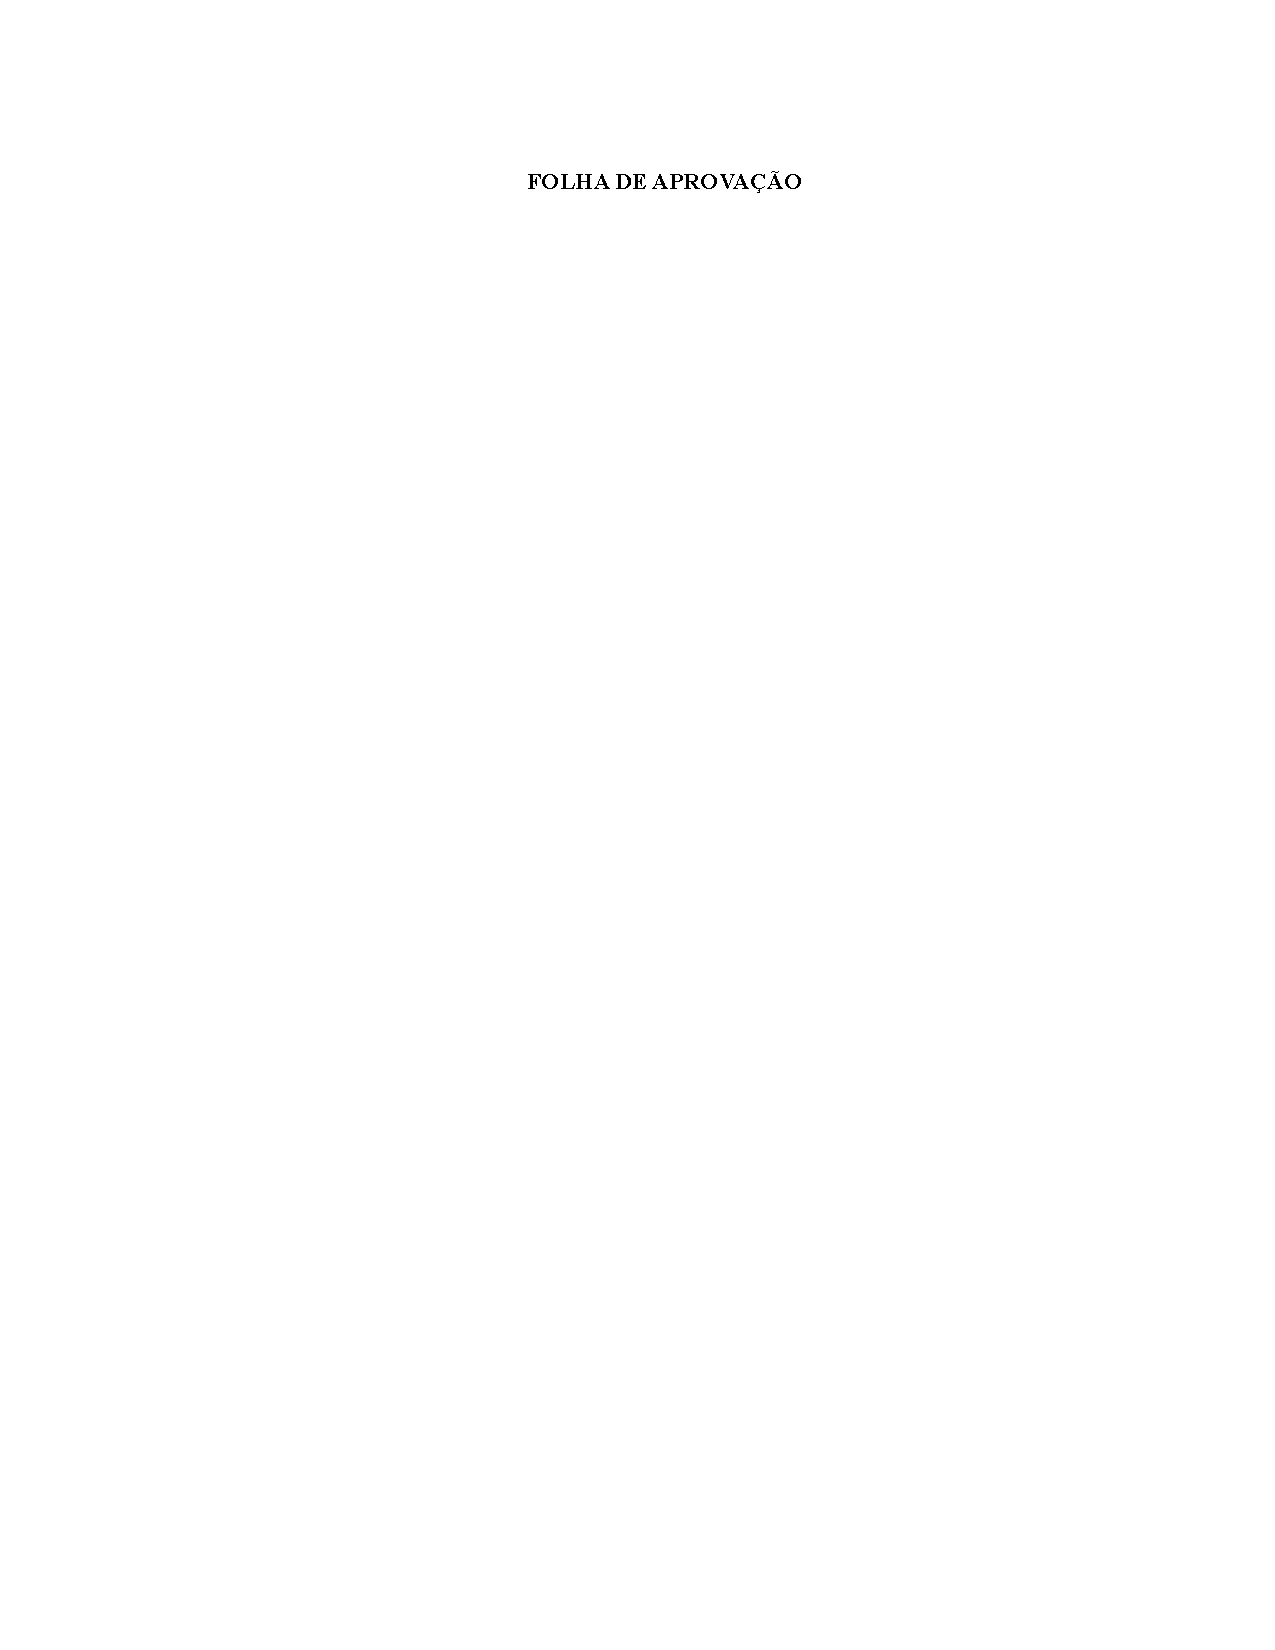
\includepdf[scale=1.0,pages=1]{./PreTexto/folha-aprovacao.pdf} % para adicionar o pdf enviado pelo professor apenas substitua o documento folha-aprovacao.pdf dentro da pasta PreTexto

%% Dedicatória
%%%% DEDICATÓRIA
%%
%% Texto em que o autor presta homenagem ou dedica seu trabalho.

\begin{dedicatoria}%% Ambiente dedicatoria

Espaço destinado à dedicatória (elemento opcional).
Folha que contém o oferecimento do trabalho à determinada pessoa ou pessoas. Exemplo:

Dedico este trabalho à minha família, pelos momentos de ausência.

\end{dedicatoria}
%% Comente para remover este item

%% Agradecimentos
%%%% AGRADECIMENTOS
%%
%% Texto em que o autor faz agradecimentos dirigidos àqueles que contribuíram de maneira relevante à elaboração do trabalho.

\begin{agradecimentos}%% Ambiente agradecimentos

Certamente estes parágrafos não irão atender a todas as pessoas que fizeram parte dessa importante fase de minha vida. Portanto, desde já peço desculpas àquelas que não estão presentes entre essas palavras, mas elas podem estar certas que fazem parte do meu pensamento e de minha gratidão. 

Agradeço ao(a) meu(minha) orientador(a) Prof.(a) Dr.(a) Nome Completo, pela sabedoria com que me guiou nesta trajetória.

Aos meus colegas de sala.

A Secretaria do Curso, pela cooperação.

Gostaria de deixar registrado também, o meu reconhecimento à minha família, pois acredito que sem o apoio deles seria muito difícil vencer esse desafio. 

Enfim, a todos os que por algum motivo contribuíram para a realização desta pesquisa.


Espaço destinado aos agradecimentos (elemento opcional). Folha que contém manifestação de reconhecimento a pessoas e/ou instituições que realmente contribuíram com o(a) autor(a), devendo ser expressos de maneira simples.

Não devem ser incluídas informações que nominem empresas ou instituições não nominadas no trabalho.

Se o aluno recebeu bolsa de fomento à pesquisa, informar o nome completo da agência de fomento. Ex: Capes, CNPq, Fundação Araucária, UTFPR, etc. Incluir o número do projeto após a agência de fomento. Este item deve ser o último.

Atenção: não utilizar este exemplo na versão final. Use a sua criatividade!

\end{agradecimentos}
%% Comente para remover este item

%% Epígrafe
%%%% EPÍGRAFE
%%
%% Texto em que o autor apresenta uma citação, seguida de indicação de autoria, relacionada com a matéria tratada no corpo do
%% Comente para remover este item

%% Resumo
%%%% RESUMO
%%
%% Apresentação concisa dos pontos relevantes de um texto, fornecendo uma visão rápida e clara do conteúdo e das conclusões do
%% trabalho.

\begin{resumoutfpr}%% Ambiente resumoutfpr
Os sistemas distribuídos desempenham um papel importante na computação moderna, pois permitem a criação de softwares escaláveis, flexíveis e de alto desempenho. Contudo, esses sistemas enfrentam instigações inerentes, como a necessidade de prover consistência, disponibilidade e tolerância a falhas de partição em um ambiente distribuído. Com isso em mente, o teorema CAP é uma importante teoria, inicialmente proposta por Eric Brewer, que lida com os trade-offs intrínsecos no design do projeto de um sistema distribuído.
O teorema CAP não é um conceito trivial então, como toda ciência, para ela evoluir, é necessário que o conhecimento desse assunto seja muito bem difundido. Sendo assim, urge a necessidade de compreender profundamente os compromissos atrelados ao teorema CAP, de modo a projetar sistemas distribuídos eficazes e adequados às necessidades específicas de cada aplicação, além de estar ciente das suas limitações.
Este artigo tem como objetivo incluir novos pesquisadores na área de modo a incitar o estudo de novos métodos e soluções. Para tanto, o teorema CAP precisa ser apresentado para os iniciantes na área da computação, comparando diferentes resultados e suas implicações em sistemas distribuídos. Dessa forma, é essencial a leitura das principais obras existentes sobre o tema, de modo a promover uma base sólida de conhecimento e estimular futuras pesquisas e inovações nesse campo em constante evolução. 
A pesquisa será conduzida por meio de uma revisão sistemática da literatura, com base em artigos científicos relevantes sobre sistemas distribuídos e o teorema CAP. Serão considerados estudos de caso e experiências práticas de implementação de sistemas distribuídos para enriquecer a compreensão dos desafios e soluções associadas ao teorema CAP. 
Espera-se que este estudo proporcione um melhor entendimento sobre o teorema CAP e suas implicações na concepção de sistemas distribuídos. Os resultados deverão apresentar uma visão clara dos compromissos envolvidos e das possíveis estratégias para alcançar consistência, disponibilidade e tolerância a partições.
Com base na análise e comparação das abordagens estudadas, espera-se que o artigo conclua que o leitor tenha compreendido por completo o teorema CAP e suas implicações, de modo a estar apto, no processo de desenvolvimento de um sistema distribuído, priorizar critérios de acordo com as necessidades e características específicas de cada aplicação, estando ciente das suas limitações. 
\end{resumoutfpr}
%% Comente para remover este item

%% Abstract
%%%% ABSTRACT
%%
%% Versão do resumo para idioma de divulgação internacional.
%% Comente para remover este item

%% Lista de algoritmos
%\incluirlistadealgoritmos%% Comente para remover este item

%% Lista de ilustrações
\incluirlistadeilustracoes%% Comente para remover este item

%% Lista de abreviaturas, siglas e acrônimos
\incluirlistadeacronimos{glossaries}%% Opções: "glossaries" (pacote) ou "file" (arquivo) ou "none" (desabilita)

%% Lista de símbolos
\incluirlistadesimbolos{nomencl}%% Opções: "nomencl" (pacote) ou "file" (arquivo) ou "none" (desabilita)

%% Sumário
\incluirsumario%% Comente para remover este item

%% Formatação de páginas de elementos textuais
\textual%% Não comente esta linha

%% Parte
% \part{Introdução}%% Comente para remover este item

%% Capítulo introdução - obrigatório
%%%% CAPÍTULO 1 - INTRODUÇÃO
%%
%% Deve apresentar uma visão global da pesquisa, incluindo: breve histórico, importância e justificativa da escolha do tema,
%% delimitações do assunto, formulação de hipóteses e objetivos da pesquisa e estrutura do trabalho.

%% Título e rótulo de capítulo (rótulos não devem conter caracteres especiais, acentuados ou cedilha)
\chapter{Introdução}\label{cap:introducao}

Os sistemas distribuídos desempenham um papel fundamental em nossa sociedade cada vez mais conectada, permitindo a troca de informações e o compartilham
ento de recursos entre diferentes dispositivos e usuários. No entanto, a natureza distribuída desses sistemas apresentam desafios significativos, como manter a consistência dos dados em ambientes onde ocorrem falhas e partições de rede. Nesse contexto, o Teorema da \gls{cap} tem sido amplamente discutido e estudado como um importante princípio para projetar e entender sistemas distribuídos, visto que veio de encontro com os conceitos de ACID(Consistência) e BASE(Disponibilidade) \cite{ConsistencyInACIDAndCAPTheoremStackOverFlow2013}.

Ao longo dos anos, diversos estudos têm explorado os desafios e soluções relacionados ao \gls{cap} em sistemas distribuídos como, por exemplo, no estudo \textit{CAP Twelve Years Later: How the ``Rules'' Have Changed} \cite{BrewerTwentyYearsLaterEricBrewer2012} do próprio criador do teorema mencionado, o qual é analisado alguns acontecimentos relacionado a má interpretação das ``regras''    do \gls{cap}. Pesquisadores têm analisado diferentes aspectos, como as propriedades dos sistemas que podem ser garantidas simultaneamente, a complexidade dos algoritmos de consistência, os trade-offs entre consistência e disponibilidade, e as estratégias para lidar com partições de rede. Várias abordagens têm sido propostas, como os modelos de consistência eventual \cite{EventuallyConsistentWernerVogels2009}, forte e fraca, além de técnicas de replicação de dados e algoritmos de consenso distribuído, como o algoritmo Paxos \cite{PaxosMadeSimpleLamport2001}.

Apesar dos avanços significativos alcançados na área, há uma lacuna no estado-da-arte em relação à difusão e compreensão do \gls{cap} entre os novos pesquisadores. A complexidade inerente ao teorema e a falta de materiais didáticos e recursos de aprendizagem adequados podem dificultar a entrada de novos estudiosos nesse campo. Portanto, é necessário direcionar esforços para preencher essa lacuna e incentivar a pesquisa nessa área vital dos sistemas distribuídos.

O objetivo deste trabalho é demonstrar a importância do \gls{cap} em sistemas distribuídos e fornecer uma revisão sistemática dos princípios relacionados a esse teorema. Busca-se enriquecer a compreensão dos desafios e soluções associados ao \gls{cap}, a fim de incentivar e capacitar novos pesquisadores a contribuírem nessa área de pesquisa. Ao final deste trabalho, espera-se que os leitores tenham adquirido conhecimento aprofundado sobre o \gls{cap}, seus conceitos fundamentais e as abordagens existentes para lidar com as suas implicações. Como objetivos específicos, ou sejam, subprodutos que contribuem para atingir o objetivo geral do artigo, temos:
\begin{itemize}
    \item Analisar e compreender os conceitos fundamentais do \gls{cap} em sistemas distribuídos, incluindo as propriedades de consistência, disponibilidade e tolerância a partições de rede.
    \item Realizar uma revisão sistemática da literatura sobre o \gls{cap}, identificando as principais abordagens, modelos de consistência e algoritmos de replicação de dados utilizados na área.
    \item Investigar os desafios e trade-offs associados à aplicação do \gls{cap} em diferentes cenários de sistemas distribuídos, considerando aspectos como escalabilidade, desempenho e resiliência a falhas.
    \item Demonstrar, por meio de exemplos e estudos de caso, a importância e os benefícios
de projetar sistemas distribuídos levando em consideração os princípios do \gls{cap}.
Contribuir para a ampliação do conhecimento na área de sistemas distribuídos, oferecendo uma visão atualizada dos avanços recentes e das tendências futuras relacionadas ao \gls{cap}.
\end{itemize}

A metodologia adotada neste trabalho consiste em uma revisão bibliográfica da literatura sobre o \gls{cap} e seus princípios. Serão pesquisados artigos científicos, livros, conferências e recursos online relevantes, selecionando-se aqueles que abordam diretamente o \gls{cap} e suas aplicações ou conceito incompreendidos em sistemas distribuídos. A partir da análise desses materiais, serão extraídos os principais resultados publicados na área, proporcionando uma visão abrangente e atualizada do estado-da-arte.


Espera-se que este trabalho proporcione uma visão abrangente dos principais resultados publicados no campo do \gls{cap} em sistemas distribuídos. Serão apresentados os diferentes modelos de consistência, as técnicas de replicação de dados mais utilizadas e os algoritmos de consenso.

O trabalho identifica e aborda uma lacuna existente na compreensão e difusão do \gls{cap} entre novos pesquisadores. Ao fornecer uma introdução clara e acessível ao tema, busca incentivar o envolvimento e a pesquisa nesse campo. Além disso, o artigo realiza uma revisão sistemática da literatura sobre o \gls{cap}, fornecendo uma compilação abrangente dos principais resultados e abordagens na área. Isso oferece uma visão consolidada e atualizada do estado-da-arte.%% Comente para remover este item

%% Capítulo
% ATENÇÃO - veja com o seu orientador se você vai ter este capítulo e se este vai ter nome!
\chapter{Revisão da Bibliográfica}
\label{cap:trabalhos:relacionados}
Uma revisão bibliográfica é necessária, pois aqui serão apresentados os conceitos básicos e fundamentais para a visão geral da área de pesquisa e do problema, porém agora com uma fundamentação teórica do assunto. A subseção de trabalhos relacionados listará as propostas relevantes, as quais serão comparadas com o trabalho em questão.

\section{Fundamentação teórica}

O Teorema CAP foi criado por Eric Brewer, o qual é muito bem definido no artigo ``Brewer's CAP Theorem'' \cite{BrewerCAPTheoremSimonSalome} explica que ``The CAP theorem states: You can have at most two of these properties for any shared-data system'', ou seja, o autor descreveu que em um sistema distribuído, é impossível garantir simultaneamente consistência, disponibilidade e tolerância a partições de rede. Esses três atributos são muito bem definidos com profundida no artigo ``Perspectives on the CAP Theorem'' \cite{PerspectivesCAPTheoremGilbertLynch2012}.

O primeiro termo da sigla \gls{cap}, denominado de ``consistência'', refere-se à uniformidade dos dados em um sistema distribuído. Um sistema é considerado consistente quando todas as réplicas dos dados em diferentes nós apresentam a mesma versão dos dados em um determinado momento.
O segundo termo da sigla trata da `availability'', que em português significa ``disponibilidade'', o qual diz respeito à capacidade de um sistema de responder a solicitações, mesmo em face de falhas ou partições de rede. Um sistema é considerado disponível se os usuários podem acessar e obter respostas, mesmo que alguns nós ou conexões falhem. Por fim, a última letra referente ao teorema trata da ``partition tolerance'', que é dado como a tolerância a partições de rede, o qual concerne à capacidade de um sistema de continuar operando e garantir consistência e disponibilidade mesmo que ocorram falhas de comunicação entre nós.
A compreensão desses conceitos é essencial para compreender os desafios e as soluções relacionados ao Teorema CAP em sistemas distribuídos.

Tais definições estão muito bem explicadas nas literatura e são mencionadas em diversos estudos, como nos artigos ``Brewer's CAP Theorem'' \cite{BrewerCAPTheoremSimonSalome}, ou no blog post ``You Can’t Sacrifice Partition Tolerance'' \cite{YouCantSacrificePartitionToleranceCodaHale2010}, sendo que o autor cita o autores Seth Gilbert e Nancy Lynch do artigo ``Perspectives on the CAP Theorem''.

\section{Trabalhos Relacionados}
Note: Comparar todos com o meu trabalho!

\begin{itemize}
    \item "Perspectives on the CAP Theorem" \cite{PerspectivesCAPTheoremGilbertLynch2012}: Este trabalho oferece uma análise abrangente das diferentes perspectivas e interpretações do Teorema CAP. Ele explora as implicações teóricas e práticas do Teorema e discute as compensações necessárias para contextos onde prioriza-se consistência ou disponibilidade em sistemas distribuídos, além disso inclui um capítulo relevante onde ele demonstra como atingir tanto consistência quanto disponibilidade, por meio da segmentação de dados, usuário, operações, entre outros. Além disso, os autores deste artigo são os responsáveis pela prova formal do \gls{cap} no artigo ``Brewer's Conjecture and the Feasibility of Consistent Available Partition-Tolerant Web Services'' \cite{Brewer'sConjectureAndTheFeasibilityOfConsistentAvailablePartition-TolerantWebServicesGilbertLynch2002}.
    \item "You Can't Sacrifice Partition Tolerance" \cite{YouCantSacrificePartitionToleranceCodaHale2010}: Este blog post enfatiza a importância da tolerância a partições de rede no contexto do Teorema CAP. Ele argumenta que a tolerância a partições é um requisito fundamental para sistemas distribuídos resilientes e explora as implicações dessa escolha como, por exemplo, em sistemas reais, é impossível atender a trilhões de requisições simultâneas tendo um arquitetura centralizada, ou seja, que não seja particionada na rede (argumento também exposto em ``Eventually Consistent'' \cite{EventuallyConsistentWernerVogels2009}. Além disso, o próprio autor do teorema CAP usou este blog post como motivação para escrever o artigo abaixo, devido ao fato do \gls{cap} ter apresentado várias interpretações errôneas.
    \item "Brewer's CAP Theorem" \cite{BrewerCAPTheoremSimonSalome}: Neste trabalho, o autor apresenta o Teorema CAP, mencionando as três propriedades (consistência, disponibilidade e tolerância a partições) definidas por outros autores e sua relação mútua. O artigo oferece uma visão geral do Teorema e suas implicações práticas, além de mencionar a formulação feita pelo Eric Brewer no artigo ``CAP Twelve Years Later - How the 'Rules' Have Changed'' de que a decisão não é binária. Por fim, o autor também menciona \cite{Brewer'sConjectureAndTheFeasibilityOfConsistentAvailablePartition-TolerantWebServicesGilbertLynch2002}, junto com exemplos de aplicações reais, como o Amazon Dynamo, do teorema em questão. 
    \item "CAP Twelve Years Later - How the 'Rules' Have Changed" \cite{TwentyYearsLaterEricBrewer2012}: Esse trabalho revisita o Teorema CAP após doze anos de sua formulação inicial. Ele discute como as interpretações erroneas do Teorema evoluíram e como as tecnologias e práticas de sistemas distribuídos se adaptaram ao longo do tempo. 
    
\end{itemize}
Em comparação com esses trabalhos relacionados, o artigo proposto "Teorema CAP em Sistemas Distribuídos: Uma Revisão Sistemática dos Princípios" busca preencher a lacuna existente na compreensão e difusão do Teorema CAP, oferecendo uma revisão sistemática da literatura sobre o tema. Ele se concentra em fornecer uma visão geral abrangente, identificar lacunas na pesquisa e apresentar recomendações práticas para a aplicação do Teorema CAP em sistemas distribuídos.

Uma lacuna que nenhum dos trabalhos acima preenche, no qual este trabalho pretende resolver, é também englobar a questão do porque a maioria dos sistemas se encontram no campo AP, ou seja, focados em ter disponibilidade e tolerância a partição. Além disso, também considero uma lacuna a ser preenchida, de modo a dar mais completude para o artigo, explica também porque a decisão não é binária e o motivo de ser inviável fugir da partição de rede. Dessa forma, o leitor tendo um artigo mais completo sobre o tema, o qual define tantos os termos, quantos as limitações e as práticas 

Essa revisão da literatura permite contextualizar o trabalho em relação aos conhecimentos existentes, destacando sua contribuição específica para o campo do Teorema CAP em sistemas distribuídos.


%---------------------------------------------------%

%% Comente para remover este item

%% Capítulo
\chapter{Desenvolvimento}\label{cap:proposta}
Na seção de desenvolvimento deste artigo, exploraremos a proposta deste instrumento de estudo, junto com uma descrição melhor da descrição do método, uma explicação dos resultados esperados e, por fim, o cronograma de execução deste estudo.

\section{Proposta}
O objetivo principal deste trabalho é realizar uma revisão sistemática da literatura sobre o teorema CAP em sistemas distribuídos, a fim de fornecer uma compreensão aprofundada dos princípios subjacentes, dos trade-offs e das estratégias para lidar com os desafios de consistência e disponibilidade, de modo a introduzir novos pesquisadores na área. Os objetivos específicos são:
\begin{itemize}
    \item Apresentar uma visão geral do Teorema CAP, incluindo suas definições e implicações para sistemas distribuídos.
    \item Realizar uma revisão bibliográfica abrangente, buscando artigos científicos, livros, conferências e recursos online relevantes que abordem o teorema CAP e seus aspectos relacionados.
    \item Analisar e comparar os trabalhos encontrados, identificando as principais abordagens e soluções propostas para lidar com os compromissos do teorema CAP.
    \item Investigar estudos de caso e experiências práticas de implementação de sistemas distribuídos, a fim de enriquecer a compreensão dos desafios e soluções associados ao teorema CAP.
    \item Identificar lacunas na literatura e destacar possíveis áreas de pesquisa futura relacionadas ao teorema CAP em sistemas distribuídos.
\end{itemize}

\section{Metologia}
A metodologia a ser adotada para o desenvolvimento deste trabalho será baseada em uma revisão sistemática da literatura. As etapas a serem seguidas são:
\begin{enumerate}
    \item Definição dos critérios de busca: serão estabelecidos critérios de busca claros, incluindo palavras-chave e filtros para selecionar os artigos relevantes para a revisão.
    \item Seleção dos artigos: os artigos serão selecionados com base em critérios de inclusão e exclusão pré-definidos, considerando sua relevância para o tema de estudo.
    \item Análise dos artigos: os artigos selecionados serão analisados em detalhes, identificando os principais conceitos, abordagens, trade-offs e resultados apresentados.
    \item Síntese dos resultados: os resultados serão sintetizados em uma revisão sistemática, organizando os principais pontos discutidos nos artigos e identificando lacunas na literatura.
\end{enumerate}

\section{Resultados e Contribuições Esperadas}
Espera-se que este trabalho proporcione uma visão abrangente dos princípios do teorema CAP em sistemas distribuídos, destacando os trade-offs e desafios associados à consistência e disponibilidade. Além disso, espera-se identificar soluções e abordagens propostas na literatura para lidar com os compromissos do teorema CAP. As principais contribuições deste trabalho são:

\begin{itemize}
    \item Revisão sistemática da literatura sobre o teorema CAP em sistemas distribuídos.
    \item Análise comparativa das abordagens e soluções encontradas na literatura.
    \item Identificação de lacunas na pesquisa atual e sugestão de possíveis áreas de pesquisa futura.
    \item Disponibilização de um artigo de referência para profissionais e pesquisadores interessados no tema.
\end{itemize}

\section{Cronograma de Execução}
O cronograma proposto para a execução deste trabalho segue as etapas definidas na metodologia, todavía é necessário acrescentar as seguintes atividades:

        5. Redação do artigo final.  
        
        6. Revisão e formatação.
        
\begin{center}
\begin{tabular}{||c c c c c c c c c c c c c||} 
 \hline
Atividade & 01/02 & 03/04 & 05/06 & 07/08 & 09/10 & 11/12 & 13/14 & 15/16 & 17/18 & 19/20 & 21/22 & 23/24\\ [0.5ex] 
 \hline\hline
 1 & X & X & X & X & X & X & X & X & X & & & \\ 
 \hline
 2 & & X & X & X & X & X & X & X & X & & & \\
 \hline
 3 & & & & X & X & X & X & X & X & & & \\
 \hline
 4 & & & & X & X & X & X & X & X & & & \\
 \hline
 5 & & & & & & X & X & X & X & X & X & \\
 \hline
 6 & & & & & & X & X & X & X & X & X & X \\
 \hline
\end{tabular}
\end{center}

Este cronograma tem uma duração total de 24 semanas, considerando uma dedicação média de 10 horas por semana.%% Comente para remover este item

%% Formatação de páginas de elementos pós-textuais
\postextual%% Não comente esta linha

%% Arquivos de referências
\arquivosdereferencias{%% Arquivos bibtex sem a extensão .bib e separados por vírgula - Não comente esta linha
  %./PosTexto/exemplos-referencias,%% Arquivo de referências - Comente para remover este item
  main%% Arquivo de referências - Comente para remover este item
}%% Não comente esta linha

%% Fim do documento
\end{document}%% Não comente esta linha
